
\documentclass[12pt,a4paper,twoside,openright]{report}

\usepackage[T1]{fontenc}
\usepackage{mathptmx}
\usepackage{amsmath,amssymb,amsfonts}
\usepackage{setspace}
\usepackage[top=1in,bottom=1in,left=2cm,right=2cm]{geometry}
\usepackage{graphicx}\graphicspath{{imgs/}}
\usepackage{subcaption}
\usepackage[sort&compress]{natbib}
\usepackage[hidelinks]{hyperref}
\usepackage{indentfirst}

\usepackage{titlesec}
\usepackage{lipsum}

\titleformat{\chapter}[display]
  {\normalfont\bfseries}{}{0pt}{\Huge}

\usepackage{fancyhdr} 
\pagestyle{fancy}
\fancyhf{}
\fancyhead[RE]{\it{\nouppercase{\leftmark}}}
\fancyhead[LO]{\it{\nouppercase{\rightmark}}}
\fancyhead[LE,RO]{\thepage}
\fancyfoot{}

\usepackage{emptypage}
\usepackage[nottoc]{tocbibind}

\setcounter{secnumdepth}{3}
\setcounter{tocdepth}{3}

\title{A Study of Properties of Open Star Clusters}
\author{Shanmugha Balan S V \\ 2019B5A30571P \\[1cm]\\{\small Advisor: Dr Kaushar Vaidya}\\[1cm]}
\date{
\includegraphics[scale=0.1]{logo} \\ Department of Physics\\ Birla Institute of Science and Technology, Pilani\\[5mm] \today}

\raggedbottom

\begin{document}

\pagestyle{empty}

\maketitle	
\cleardoublepage

\singlespacing
\pagenumbering{roman}
\pagestyle{plain}
	
\begin{abstract}
Gaia is an astrometry mission by the ESA, which has helped in cataloguing numerous objects in our galaxy in unprecedented detail. The cluster membership information based on Gaia DR2 data of open clusters will be used to understand the effect of dynamical evolution on the observed properties of star clusters. In particular, star clusters with a clear binary track are examined to study the radial distributions of these binary stars with respect to the radial distribution of single stars. Alongside, the morphology of star clusters is examined to look for the presence of any tidal tails in the star clusters. 
\end{abstract}	

\cleardoublepage
\pagestyle{fancy}
	
\tableofcontents

\cleardoublepage
\singlespacing
\pagenumbering{arabic}	

%================ch1======================================
\chapter{Introduction}\label{ch:ch1}

\section{Gaia Mission}
We have come a long way in observing the skies, from the naked eye to the mural instrument, from telescopes to space missions. The Gaia mission \citep{gaia} \citep{gaiafaccs} is one such astrometry mission launched in 2013. The spacecraft aims to measure the positions, distances and motions of celestial objects, not just in our galaxy but much beyond. The mission aims to be the most precise 3D catalogue of the sky, mapping every object it can while also measuring their motions which can give clues about the origin and evolution of our galaxy, the Milky Way.

The mission aims to determine the position and parallax of around a billion stars to an accuracy of around 20 $\mu as$. The catalogue is set to be released in stages. The first data release took place in 2016 \citep{gaiadr1}, based on 14 months of observation. It inlcuded the positions and magnitudes for over a billion stars using only Gaia data. The second data release took place in 2018 \citep{gaiadr2}, after 22 months of observations, and improved on the precision of the previous release, as well as adding parallaxes and proper motions.

\section{Star Clusters}
Gravity is one of the 4 fundamental forces which keeps large celestial structures in place. A star cluster is a gravitationally bound group of stars. They share a common origin and provide a way to study stellar evolution. They can be globular or open.

\subsection{Globular Clusters}
A globular cluster is a roughly spherical collection of stars orbiting the galactic core. They have a dense concentration of stars in their centers and are thinly spread out further from the center in the halo. They are composed of thousands of low metal stars. They are generally found in the halo of a galaxy and are generally older than the stars in open clusters. \citep{globclust} The proportion of metals, called metallicity, is rather low in these stars. The metallicity of a star is an indicator of its age, and the low metallicity of stars in globular clusters shows this. \citep{introstars}

\subsection{Open Clusters}
An open cluster is a group of a few thousand stars formed from the same molecular cloud. They are named so because often individual component stars can be resolved rather easily with a telescope. They are generally found in the disc of the galaxy. They are rather loosely bound by gravitational attraction between the member stars. Gravitational effects from other massive bodies as it moves on its journey around the center of the galaxy often disperse the order of these clusters. They are much younger compared to globular clusters, some even showing signs of nebulosity. Properties of the cluster members can be determined easily because they have are at the same distance away from us and they have a similar age and chemical composition \citep{openclust}. This will also be the focus of this report.

\section{Gaia Data for Open Clusters}
While the Gaia mission provided us with very precise data regarding astronomical objects, they are not classified. The study by Cantat-Gaudin et. al \citep{cg} aims to determine a list of members of open clusters and derive mean parameters from them using Gaia data. They obtained a list of 1229 open clusters with associated members and cluster parameters. The cluster members identified by Cantat-Gaudin are available on the VizieR database \citep{vizier}, which is used for this study. The data lists the positions of the clusters and their members, with parallaxes, proper motions and color magnitudes. From the other Gaia data, more information can be queried for individual stars. Combining the data, the properties of these star clusters can be studied. Eventually, we can separate the binary stars from the single ones and study their radial distributions. We can then examine their evolution and morphology.

\section{Photometry}
The art of measuring the electromagnetic radiation from a point source in the sky is known as photometry. Thus, we can use this information to calculate the distance to an object, its mass, its temperature and chemical composition. To determine some of these factors, we will plot a very useful graph known as a Hertzsprung-Russel chart or a color magnitude diagram.


\subsection{Color Magnitude Diagrams}
To study about the life cycles of stars, their evolution, we plot the luminosities of stars against their color. This is essentially a plot of the total energy given by a star against the surface temperature. This is known as a Hertzsprung-Russel diagram (HR diagram) or a color magnitude diagram (CMD). There are four major groups of stars in this plot. The smear in the bottom left representing the white dwarfs. They are among the older stars in the life cycle and most open clusters don't have them. They undergo hydrogen fusion and take up the bulk of a star's life. The horizontal branch breaking away from the main sequence corresponds to the red giant stars and the top right belongs to the supergiants. There are other minor divisions in the clusters, such as blue stragglers as well.  \citep{introstars}

\begin{figure}[H]
	\centering
	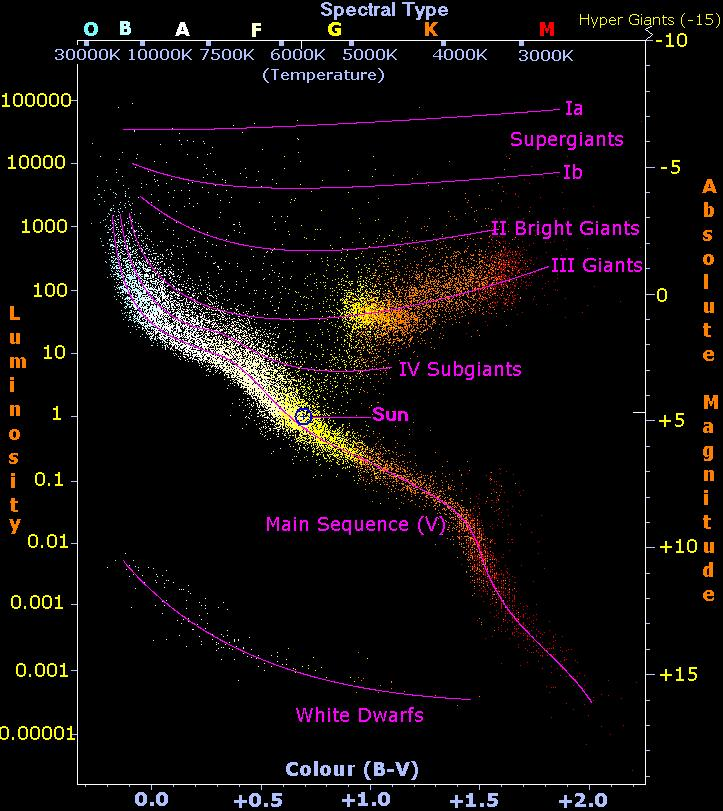
\includegraphics[width=0.6\linewidth]{hr-diagram.jpg}
	\caption{H-R Diagram \citep{wimecommons}}
	\label{fig:image1}
\end{figure}

\subsection{Isochrones}
A stellar isochrone is a curve on the color magnitude diagram indicating a population of stars of the same age. They can be used to date stars in open clusters because they all approximately have the same age. Isochrone data is available in the internet and they can be downloaded to test which one gives the best fit. The best fitting isochrones don't just reveal the age of the cluster, but much more information.




%================ch2======================================
\chapter{Processing the data}\label{ch:ch2}

\section{Collecting Star Cluster Data}
Initially the data from Gaia is queried from the VizieR database \citep{vizier}. The results obtained by Cantat-Gaudin \citep{cg} can be obtained in a tabular form. Hence we obtain the data for 1229 clusters. The database enables us to access position, motion, cataloguing and color information. We require only the photometric data - the color magnitude and the photometric magnitude for the first part. This data was scraped from the website. This enables us to plot a color magnitude diagram for all the clusters. The membership probability was considered and stars with a threshold probability of more than $0.7$ were highlighted. The plots of these clusters were analysed, and nine clusters (IC 4651, IC 4756, NGC 752, NGC 1664, NGC 2281, NGC 2287, NGC 2527, NGC 6281, NGC 6405) were shortlisted for further analysis.

\begin{figure}[h]
	\centering
	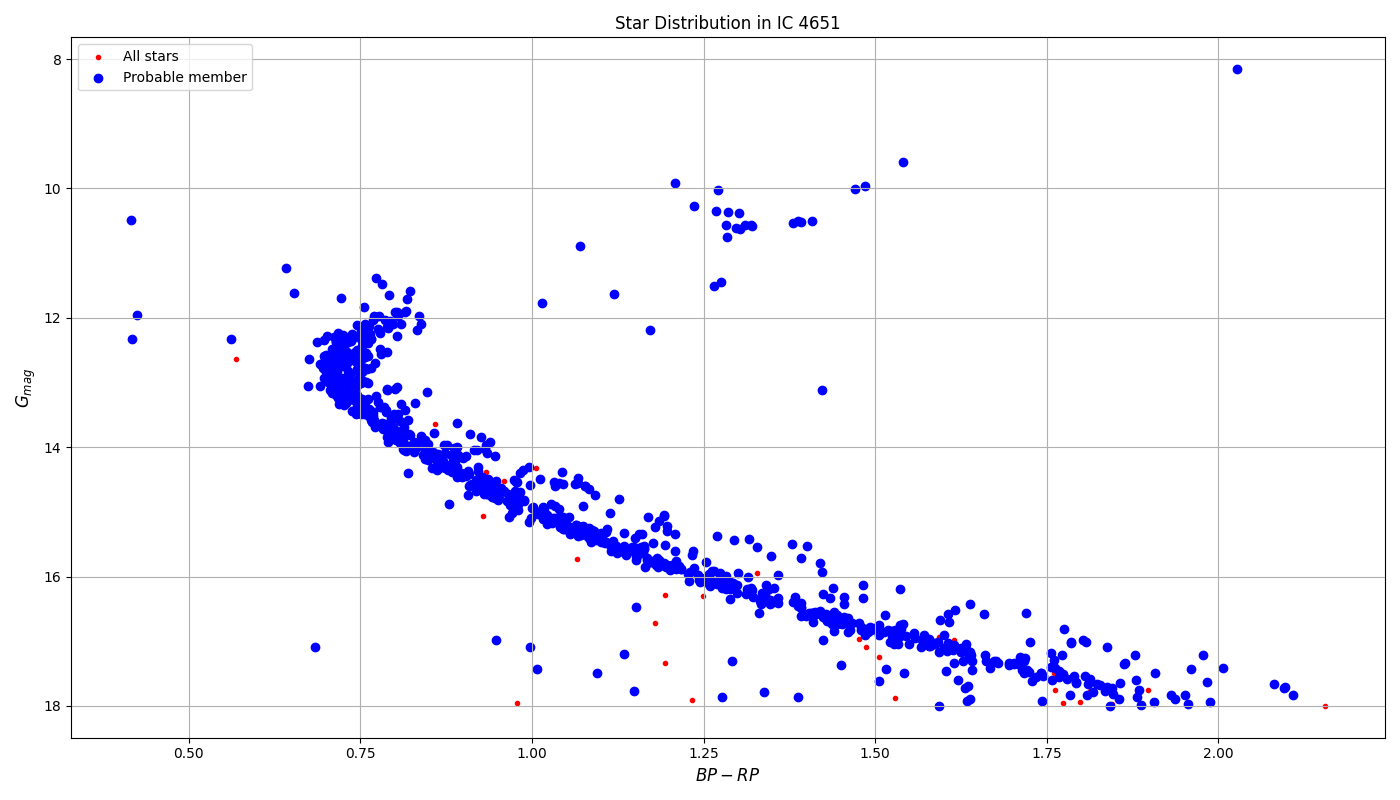
\includegraphics[width=0.8\linewidth]{IC 4651.png}
	\caption{CMD for the cluster IC 4651}
	\label{fig:im2}
\end{figure}

In each of these plots, two tracks can be observed. One is a thick lower track and there is a slightly sparse track above it. These correspond to single stars and stars in a binary system. These were separated and classified into their categories. To separate the two tracks, an isochrone was fitted to each cluster selected. This isochrone was then duplicated and shifted up by a certain value. The stars in between the isochrone and its twin are the single stars and the stars above the twin are the binary stars.

\section{Collecting Isochrone Data}
The data for isochrones is available in the CMD database \citep{cmdSite}. It provides interpolated isochrones. This photometry can be used for studying the clusters we have at hand. We also need distance, metallicity and age to plot the ischrone. This data is available for all clusters in this study from the WEBDA database \citep{webda} or from a literature survey on NASA's ADS. To plot the cluster data and isochrone together, we need to process the isochrone data. To do this, we must find out the extinction coefficient ($A_g$) for the data. The mean and median value for this is calculated from the downloaded cluster data and varied to find the best fit isochrone. Also found are the mean and median values for $E_{BP-RP}$ from the cluster data. Now, the magnitude data from the isochrones consist of absolute magnitudes. This is converted to apparent magnitudes, so that they can be plotted with the stars. Corrections are made for the color axis and magnitude axis to find the best fit isochrone. Then a shift value is added to the magnitude values of the isochrones' $(x,y)$ pairs so that the binary track can be separated.
$$g_{mag} = G_{mag} + 5 \log d - 5 + A_g$$
$$e_{BP-RP} = G_{BP} - G_{RP} + E_{BP-RP}$$

\begin{figure}[h]
	\centering
	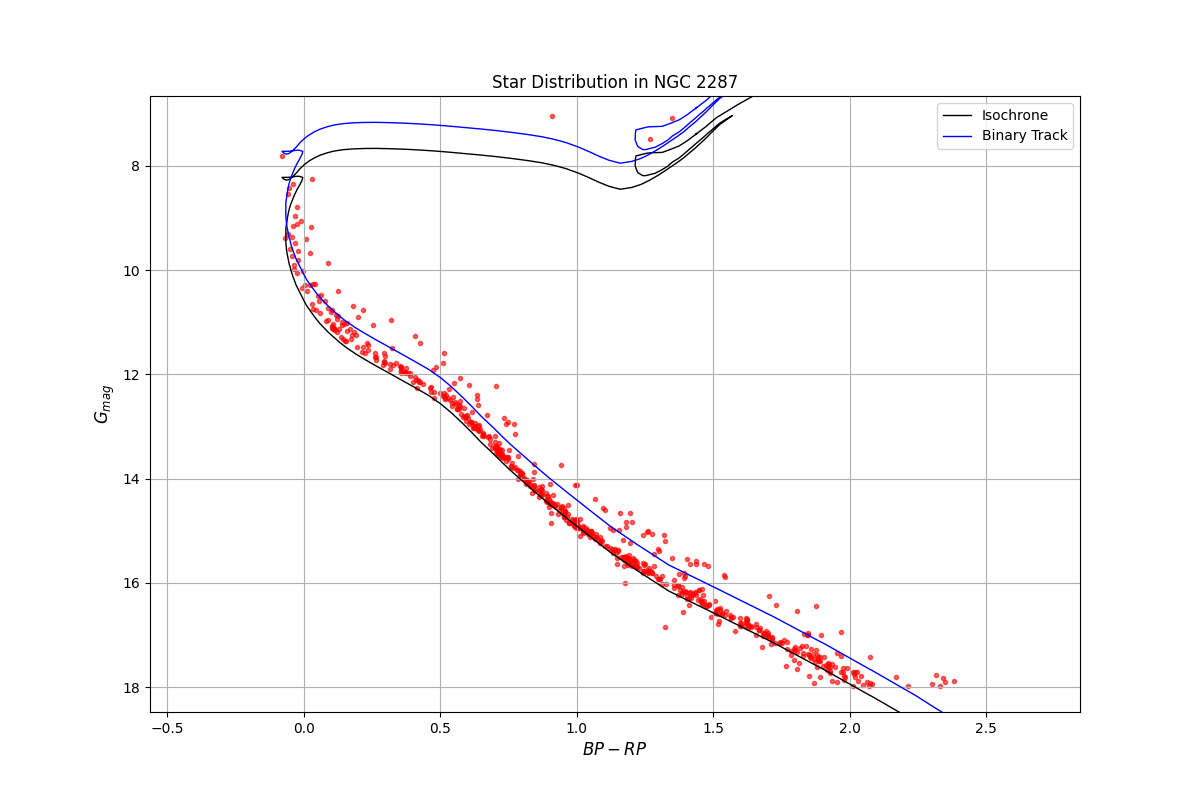
\includegraphics[width=\linewidth]{NGC 2287.png}
	\caption{CMD with the isochrone and line separating binary track for NGC 2287}
	\label{fig:im3}
\end{figure}


	
%================ch3======================================
\chapter{Analysing the data}\label{ch:ch3}

\section{Radial Distribution of Stars}
The radial distributions were calculated for each cluster individually for each track. The mean shift algorithm was used to find the center of the clusters. The celestial coordinates of the center of the cluster allows us to calculate the radial distance of every star in the cluster from its center. The \lstinline{astropy.coordinates} {}submodule has some useful classes in this regard. We can get the radial separation of these stars from the cluster center in arcminutes.

\subsection{Mean Shift Algorithm}
The mean shift algorithm is an unsupervised, non-parametric, clustering algorithm. It iteratively shifts points towards the highest density of data points - cluster centers - and classifies them accordingly. It doesn't make any assumption about the model like K-means or Gaussian mixture models. The \lstinline{scikit-learn} {}implementation was used. The model takes in a parameter - bandwidth. This bandwidth is used in the RBF kernel for the algorithm. This parameter defines how many clusters will be there in the data. Setting a relatively high value for this makes sure there is only one cluster picked up from the data. 

\subsection{Plotting the Distributions}
The calculated radial distance was plotted against the number of stars under that distance for a single track and a binary track. 

\begin{figure}[H]
\centering
\begin{subfigure}[b]{0.4\textwidth}
  \centering
  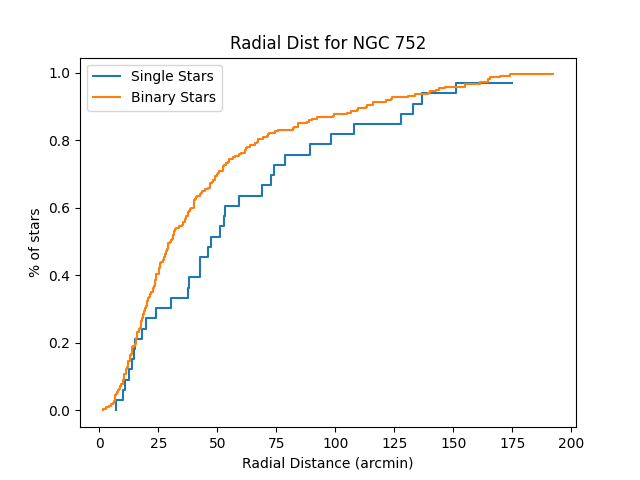
\includegraphics[width=\textwidth]{NGC 752_rad.png}
  \caption{NGC 752}
  \label{fig:im4}
 \end{subfigure}
~
\begin{subfigure}[b]{0.4\textwidth}
  \centering
  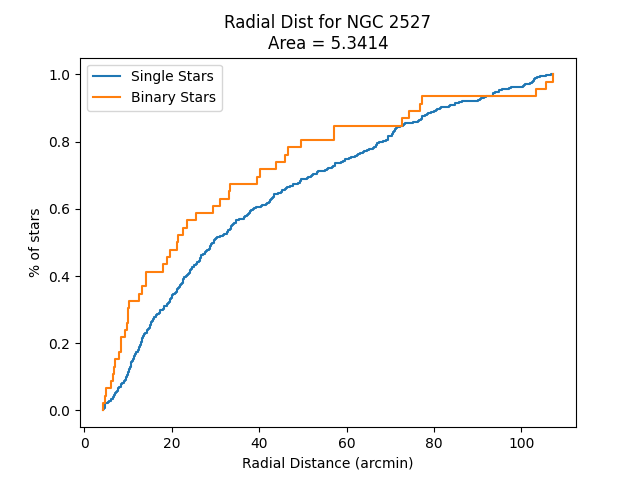
\includegraphics[width=\textwidth]{NGC 2527_rad.png}
  \caption{NGC 2527}
  \label{fig:im5}
\end{subfigure}
\caption{Radial Distribution for Star Clusters}
\label{fig:sim1}
\end{figure}

With both the tracks closer to each other at the core for NGC 752, we find that the central area of the cluster has an equal proportion of single and binary stars. From a broader perspective, we find that there are many more single stars in the cluster when the entirety is taken. The area parameter mentioned in the plot is the area between the curves of the single and binary track. However, when there are more single stars, this area is negative. The binary track is more jagged and stepped because there are many more single stars in a cluster. Nevertheless, both the curves are normalized to a percentage scale so that they can be plotted together and the area between them can be evaluated.

\section{King's Profile}
The King's profile\citep{kingprofile} is fitted for all the clusters in the study. The stars are divided into bins based on the radial distance from the cluster center. These bins are all annular rings of equal areas. This would mean the $n^{th}$ bin would be sandwiched between rings of radius $\sqrt{n-1}R$ and $\sqrt{n}R$ where $R$ is the radius of the cluster. After finding the number of stars in one bin, dividing that number by the area of the ring gives the surface density. When plotted against the radius on a log-log plot, we get a distribution of stars based on their proximities to the cluster center. Now we fit the curve given by the following equation to the data.
$$f = k \left( \frac{r_c}{\sqrt{r^2+r_c^2}} - \frac{r_t}{\sqrt{r_c^2+r_t^2}} \right) ^2$$
$k$ is an amplitude or a scaling factor, which is simply the surface density of the innermost bin. $r_c$ is the core radius and $r_t$ is the tidal radius.  $r_c$ and $r_t$ are the variable parameters which can be modified to get the best fit to the data. From the fitting procedure we can determine the core radius and tidal radius of the star cluster. The profile can be plotted easily with the \lstinline{astropy} {} module.

\begin{figure}[h]
	\centering
	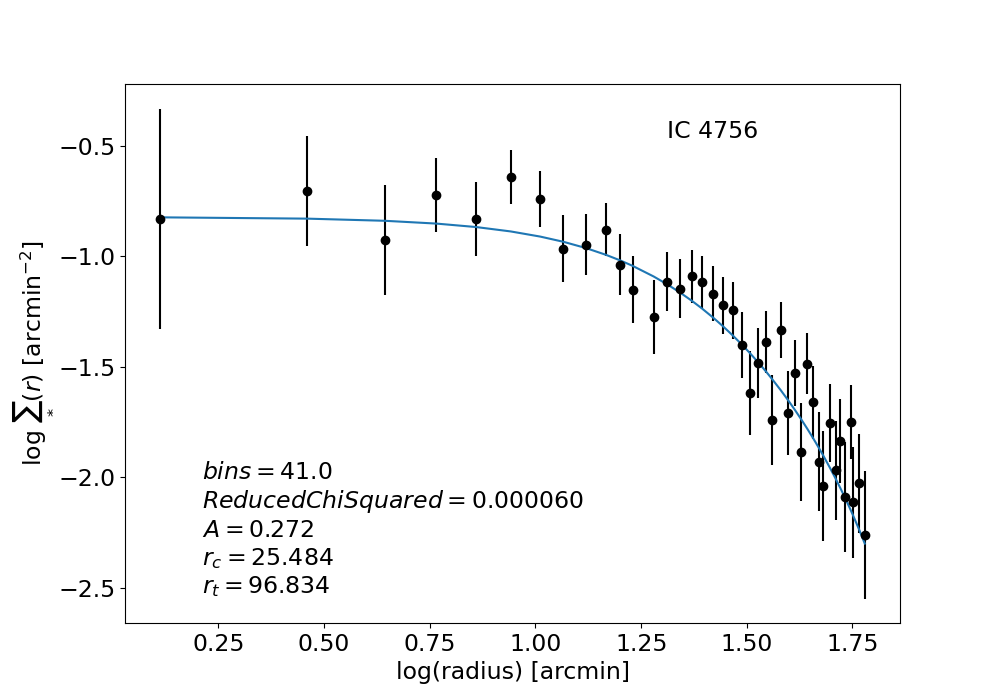
\includegraphics[width=0.7\linewidth]{IC_4756_kings.png}
	\caption{King's Profile for IC 4756}
	\label{fig:im6}
\end{figure}


\section{Determining Mass Function}
The mass of stars in the main sequence is strongly correlated with the magnitude of the stars. This relation can be found by fitting a polynomial to our data. \lstinline{numpy} {}has a submodule for dealing with polynomials and the \lstinline{polyfit} {}will fit a polynomial to the given data. In this study, we attempted to fit a cubic polynomial to approximate the relationship between magnitude and mass. 

\begin{figure}[h]
	\centering
	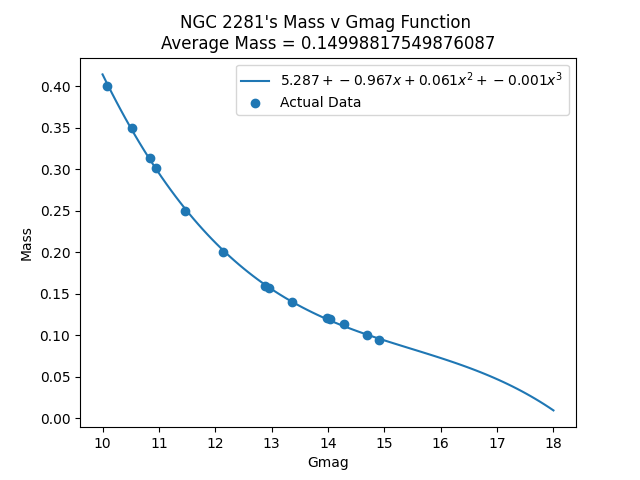
\includegraphics[width=0.6\linewidth]{NGC 2281_mass_dist.png}
	\caption{Fitting the polynomial for the isochrone of NGC 2281}
	\label{fig:im7}
\end{figure}

\subsection{Central Density}
To determine the central density, we will consider the stars in a small radius around the center of the cluster. We will first convert the radius of this region into parsecs to calculate the volume using the standard formula for the volume of a sphere. Next, we will sum up the estimated masses of all the stars in this region. This can be done by finding the mass by substituting the known magnitude values into the mass function estimated by the isochrone. Now that we have evaluated both the mass of the center and its volume, we can find the central density. Clusters with larger central density have more stars in the core and would have undergone multiple relaxations.

\section{Determing the Relaxation Time for the Clusters}
With the average mass, the number of stars in the cluster, central density and cluster radius, we have found out all the parameters we need to find the relaxation time. Relaxation time is a measure of how long an average star in a cluster can retain its initial energy. We can use this equation to evaluate the same.
$$t_{rc} = 1.491 \times 10^7 \text{yr} \times \frac{k}{\ln(0.4 N_*)} <m_*>^{-1} \rho_{M, 0}^{1/2} r_c^3$$

Finally, since all the stars along the isochrone are of similar age, we can use the isochrone age as an approximation for the age of the entire cluster. In combination with the calculated time, this allows us to identify the relaxations the cluster has undergone. This figure gives an estimate of how many relaxation periods a cluster would have undergone.

$$N_{relax} = C_{Age}/t_{rc}$$

The more relaxations a star would have undergone, the more time it would have had to ensure it settles into a final structure. External gravitational influences from some massive event or even the passing by the orbit of another large cluster might disrupt this cycle. Plotting the area between the tracks along with $N_{relax}$ might help us understand if there is a link between these structural features of a cluster.
	

\appendix	
%%================app1======================================
\chapter{Supporting Information}\label{app:app1}

\begin{figure}[h]
	\centering
	\includegraphics[width=.5\textwidth]{image2}
	\caption{Caption of image 2.}
	\label{fig: img2}
\end{figure}	

\singlespacing

\nocite{*}
\bibliographystyle{unsrt}	
\bibliography{mybib}
	
\end{document}














































